% Figure 1. The validity ladder: gate plus four levels, read bottom to top.
% Compile: tectonic fig1_ladder.tex   (standalone; natural width 6.5 in, use at 100% in the manuscript)
% Content sources (paper_brm/analysis_brm): GATE.md, L1.md, L2.md, L3.md, L4.md, method sections.
% Dependency structure: plan/DECISIONS_2026-09-26.md decision 1. L4 rules: decision 7 (margin .08, R3 a diagnostic).
% Fixes audit ledger L13: the gate sets k for levels 2 and 3 only; level 4 has an NHANES comparator;
% a level-1 failure restricts single-draw use only and stops nothing above it.
% Type: body 8 pt, small type 7.2 pt (nothing below 7 pt at 100%).
\documentclass[border={1pt 3pt 1pt 1pt}]{standalone}
\usepackage[T1]{fontenc}
\usepackage{helvet}
\renewcommand{\familydefault}{\sfdefault}
\usepackage{sansmath}
\usepackage{xcolor}
\usepackage{tikz}
\usetikzlibrary{arrows.meta,calc,fit,backgrounds}

\definecolor{acc}{RGB}{0,95,158}   % the one accent: dependencies
\definecolor{ink}{gray}{0.10}
\definecolor{mid}{gray}{0.40}
\definecolor{rule}{gray}{0.62}
\definecolor{gatefill}{gray}{0.90}

\newcommand{\smalltype}{\fontsize{7.2}{8.4}\selectfont}
\newcommand{\lvtag}[1]{{\smalltype\color{mid}\MakeUppercase{#1}}\\[-0.2ex]}
\newcommand{\nm}[1]{\textbf{#1}\\[0.3ex]}
\newcommand{\nohy}{\hyphenpenalty=10000 \exhyphenpenalty=10000 \relax}
\newcommand{\pass}{\textbf{Pass:}~}
\newcommand{\nh}{NHANES \mbox{2005--2018}}

\begin{document}
\sansmath
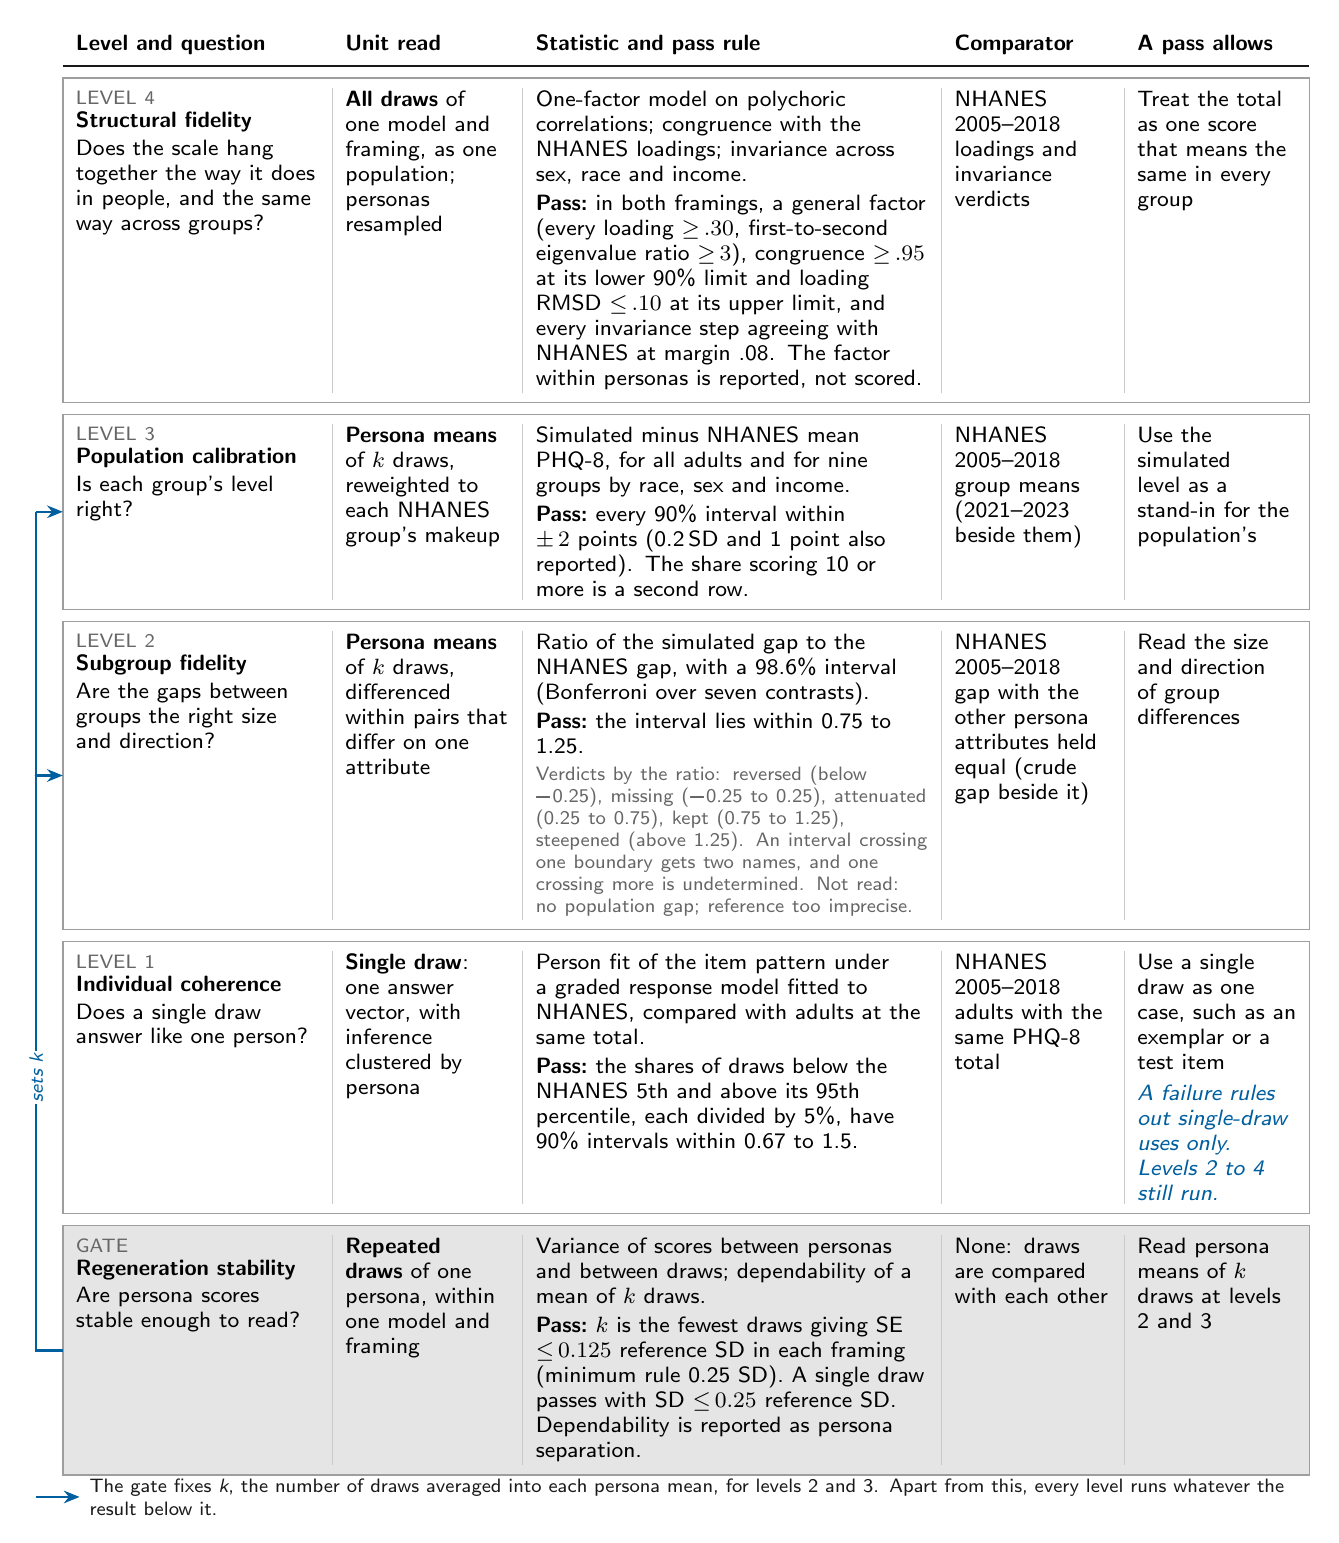
\begin{tikzpicture}[
  font=\footnotesize\color{ink},
  cell/.style={anchor=north west, align=left, inner xsep=1.6mm, inner ysep=1.5mm,
    font={\footnotesize\linespread{0.95}\selectfont\nohy}},
  cA/.style={cell, text width=31mm},
  cB/.style={cell, text width=21mm},
  cC/.style={cell, text width=50mm},
  cD/.style={cell, text width=20mm},
  cE/.style={cell, text width=20.3mm},
  hd/.style={cell, font=\footnotesize\bfseries, inner ysep=1mm},
  rowbox/.style={draw=rule, line width=0.5pt, inner sep=0pt},
  dep/.style={-{Stealth[length=2.0mm,width=1.6mm]}, acc, line width=0.9pt},
]
% column left edges (mm); x = 0 to 6 is the lane for the dependency arrows
\coordinate (xA) at (6mm,0);
\coordinate (xB) at (40.2mm,0);
\coordinate (xC) at (64.4mm,0);
\coordinate (xD) at (117.6mm,0);
\coordinate (xE) at (140.8mm,0);
\coordinate (xR) at (164.3mm,0);

% one rung = five cells top-aligned at #2, framed as one row
% #1 id, #2 top coordinate, #3-#7 cell text, #8 extra row style
\newcommand{\rung}[8]{%
  \node[cA] (#1a) at (xA |- #2) {#3};
  \node[cB] (#1b) at (xB |- #2) {#4};
  \node[cC] (#1c) at (xC |- #2) {#5};
  \node[cD] (#1d) at (xD |- #2) {#6};
  \node[cE] (#1e) at (xE |- #2) {#7};
  \node[fit=(#1a)(#1b)(#1c)(#1d)(#1e)(xR |- #2), inner sep=0pt] (#1) {};
  \begin{scope}[on background layer]
    \path[rowbox,#8] (#1.north west -| xA) rectangle (#1.south east -| xR);
    \foreach \c in {xB,xC,xD,xE}{\draw[rule!55, line width=0.3pt] (\c |- #1.north) ++(0,-1.2mm) -- ($(\c |- #1.south)+(0,1.2mm)$);}
  \end{scope}
}

% ---------- header ----------
\coordinate (top) at (0,0);
\node[hd] (ha) at (xA |- top) {Level and question};
\node[hd] (hb) at (xB |- top) {Unit read};
\node[hd] (hc) at (xC |- top) {Statistic and pass rule};
\node[hd] (hd) at (xD |- top) {Comparator};
\node[hd] (he) at (xE |- top) {A pass allows};
\draw[ink, line width=0.6pt] ($(ha.south west)+(0,-0.3mm)$) coordinate (hrule) -- (xR |- hrule);

% ---------- Level 4 ----------
\coordinate (t4) at ($(hrule)+(0,-1.6mm)$);
\rung{L4}{t4}
 {\lvtag{Level 4}\nm{Structural fidelity}Does the scale hang together the way it does in people, and the same way across groups?}
 {\textbf{All draws} of one model and framing, as one population; personas resampled}
 {One-factor model on polychoric correlations; congruence with the NHANES loadings; invariance across sex, race and income.\\[0.4ex]
  \pass in both framings, a general factor (every loading ${\geq}\,.30$, first-to-second eigenvalue ratio ${\geq}\,3$), congruence ${\geq}\,.95$ at its lower 90\% limit and loading RMSD ${\leq}\,.10$ at its upper limit, and every invariance step agreeing with NHANES at margin .08. The factor within personas is reported, not scored.}
 {\nh{} loadings and invariance verdicts}
 {Treat the total as one score that means the same in every group}
 {}

% ---------- Level 3 ----------
\coordinate (t3) at ($(L4.south)+(0,-1.6mm)$);
\rung{L3}{t3}
 {\lvtag{Level 3}\nm{Population calibration}Is each group's level right?}
 {\textbf{Persona means} of $k$ draws, reweighted to each NHANES group's makeup}
 {Simulated minus NHANES mean PHQ-8, for all adults and for nine groups by race, sex and income.\\[0.4ex]
  \pass every 90\% interval within ${\pm}\,2$ points (0.2\,SD and 1 point also reported). The share scoring 10 or more is a second row.}
 {\nh{} group means (2021--2023 beside them)}
 {Use the simulated level as a stand-in for the population's}
 {}

% ---------- Level 2 ----------
\coordinate (t2) at ($(L3.south)+(0,-1.6mm)$);
\rung{L2}{t2}
 {\lvtag{Level 2}\nm{Subgroup fidelity}Are the gaps between groups the right size and direction?}
 {\textbf{Persona means} of $k$ draws, differenced within pairs that differ on one attribute}
 {Ratio of the simulated gap to the NHANES gap, with a 98.6\% interval (Bonferroni over seven contrasts).\\[0.4ex]
  \pass the interval lies within 0.75 to 1.25.\\[0.5ex]
  {\smalltype\color{mid}Verdicts by the ratio: reversed (below \textminus0.25), missing (\textminus0.25 to 0.25), attenuated (0.25 to 0.75), kept (0.75 to 1.25), steepened (above 1.25). An interval crossing one boundary gets two names, and one crossing more is undetermined. Not read: no population gap; reference too imprecise.\par}}
 {\nh{} gap with the other persona attributes held equal (crude gap beside it)}
 {Read the size and direction of group differences}
 {}

% ---------- Level 1 ----------
\coordinate (t1) at ($(L2.south)+(0,-1.6mm)$);
\rung{L1}{t1}
 {\lvtag{Level 1}\nm{Individual coherence}Does a single draw answer like one person?}
 {\textbf{Single draw}: one answer vector, with inference clustered by persona}
 {Person fit of the item pattern under a graded response model fitted to NHANES, compared with adults at the same total.\\[0.4ex]
  \pass the shares of draws below the NHANES 5th and above its 95th percentile, each divided by 5\%, have 90\% intervals within 0.67 to 1.5.}
 {\nh{} adults with the same PHQ-8 total}
 {Use a single draw as one case, such as an exemplar or a test item\\[0.6ex]
  {\color{acc}\itshape A failure rules out single-draw uses only. Levels 2 to 4 still run.\par}}
 {}

% ---------- Gate ----------
\coordinate (t0) at ($(L1.south)+(0,-1.6mm)$);
\rung{G}{t0}
 {\lvtag{Gate}\nm{Regeneration stability}Are persona scores stable enough to read?}
 {\textbf{Repeated draws} of one persona, within one model and framing}
 {Variance of scores between personas and between draws; dependability of a mean of $k$ draws.\\[0.4ex]
  \pass $k$ is the fewest draws giving SE ${\leq}\,0.125$ reference SD in each framing (minimum rule 0.25 SD). A single draw passes with SD ${\leq}\,0.25$ reference SD. Dependability is reported as persona separation.}
 {None: draws are compared with each other}
 {Read persona means of $k$ draws at levels 2 and 3}
 {fill=gatefill}

% ---------- dependencies: the gate sets k for levels 2 and 3 only ----------
\coordinate (lane) at (2.6mm,0);
\coordinate (gy) at ($(G.north)!0.5!(G.south)$);
\draw[acc, line width=0.9pt] (xA |- gy) -- (lane |- gy) -- (lane |- L3.center);
\draw[dep] (lane |- L2.center) -- (xA |- L2.center);
\draw[dep] (lane |- L3.center) -- (xA |- L3.center);
\fill[acc] (lane |- L2.center) circle (0.55pt);
\node[rotate=90, font=\smalltype\itshape, text=acc, fill=white, inner sep=0.6pt] at (lane |- L1.center) {sets \textit{k}};

% ---------- key ----------
\coordinate (k0) at ($(G.south west)+(0,-2.8mm)$);
\draw[dep] ($(k0)+(-3.4mm,0)$) -- ($(k0)+(2.2mm,0)$);
\node[anchor=west, font=\smalltype, text=ink, inner sep=0pt, text width=154mm, align=left] at ($(k0)+(3.4mm,0)$)
  {The gate fixes \textit{k}, the number of draws averaged into each persona mean, for levels 2 and 3. Apart from this, every level runs whatever the result below it.};
\end{tikzpicture}
\end{document}
